

Schon im frühen 20. Jahrhundert begannen Meteorolog:innen zu erkennen, dass grossräumige Strömungen in der Atmosphäre nicht nur durch Temperaturunterschiede, sondern auch durch die Erdrotation beeinflusst werden \cite{https://doi.org/10.1002/wcc.95}.
Eine Schlüsselfigur in diesem Zusammenhang war Carl-Gustaf Rossby, ein schwedisch-amerikanischer Meteorologe.
In seiner Arbeit von 1939 untersuchte er den Zusammenhang zwischen der Intensität der zonalen Zirkulation und der Verschiebung der sogenannten permanenten Aktionszentren in der Atmosphäre \cite{rossby:1939relation}.
Ein Jahr später veröffentlichte er seine grundlegende Theorie der planetaren Wellenmuster in der Atmosphäre, die heute als \emph{Rossby-Wellen} bekannt sind \cite{rossby:1940planetary}.
Diese Wellen sind heute ein zentrales Konzept in der Dynamik der Atmosphäre und tragen wesentlich zum Verständnis des Wetters in den mittleren Breiten bei.

Rossby erkannte, dass die scheinbaren Kräfte, die durch die Rotation der Erde entstehen, insbesondere der \emph{Coriolis-Effekt}, eine wellenartige Bewegung grossräumiger atmosphärischer Strömungen erzeugen können.
Diese wellenförmigen Muster bewegen sich typischerweise von West nach Ost und beeinflussen massgeblich Hoch- und Tiefdrucksysteme sowie den Verlauf von Wetterfronten über Tage hinweg.

Die Untersuchung dieser Prozesse erfordert ein Verständnis physikalischer Konzepte wie der \emph{Vorticity} (Wirbelstärke), der \emph{absoluten} und \emph{potenziellen Vorticity} sowie deren Erhaltung unter bestimmten Bedingungen.
Diese Begriffe ermöglichen es, die Bewegung von Luftpaketen auf einem rotierenden Planeten mathematisch zu beschreiben und zu erklären, warum Rossby-Wellen entstehen und wie sie sich ausbreiten.

Ziel dieses Textes ist es, die Grundlagen der atmosphärischen Dynamik zu skizzieren, die zur Entstehung von Rossby-Wellen führen.
Beginnend mit der Erddrehung und dem Coriolis-Effekt, werden die Begriffe der Vorticity eingeführt und schrittweise zur potenziellen Vorticity erweitert.
Die Erhaltung dieser Grösse stellt den Ausgangspunkt für die mathematische Herleitung und das physikalische Verständnis von Rossby-Wellen dar.
Abschliessend wird ihre Rolle in typischen Wetterphänomenen beleuchtet.


\subsection{Visuelle Einführung: Rossby-Wellen im Wettergeschehen}

Zur Einführung betrachten wir zunächst ein einzelnes Kartenbeispiel 
(Abbildung~\ref{fig:rossby_atlantic_single}), das als Referenz für die Interpretation der 
folgenden Abbildungen dient. 
Die Darstellung basiert auf ERA5-Reanalysedaten des ECMWF (abgerufen über die CDS~API) 
und zeigt die atmosphärische Situation am 1.\ Mai~2025 um 00:00~UTC auf dem Druckniveau 
von 500\,hPa, das sich in der oberen Troposphäre im Bereich des Jetstreams befindet.


Die Karte nutzt eine Lambert-Conformal-Kartenprojektion mit Mittelmeridian \(-30^\circ\), zentriert auf den Atlantischen Ozean.
Der dargestellte Ausschnitt reicht von Nordamerika über den Atlantik bis nach Europa (\(-90^\circ\) bis \(30^\circ\) Länge, \(20^\circ\) bis \(75^\circ\) Breite).

Inhaltlich zeigt die Karte:
\begin{itemize}
	\item \textbf{Geopotentielle Höhenlinien} (in Metern, schwarze Linien): verbinden Punkte gleichen Druckniveaus, geben Auskunft über die grossräumige Druck- und Temperaturverteilung.
	\item \textbf{Farbflächen}: Windgeschwindigkeit in m/s.
	\item \textbf{Pfeile}: Windvektoren, deren Richtung und Länge Strömungsrichtung und -geschwindigkeit wiedergeben.
\end{itemize}

Das wellenförmige Muster der Höhenlinien und Windfelder ist charakteristisch für Rossby-Wellen, die sich von West nach Ost ausbreiten und mit Hoch- und Tiefdrucksystemen verknüpft sind.

\begin{figure}
	\centering
	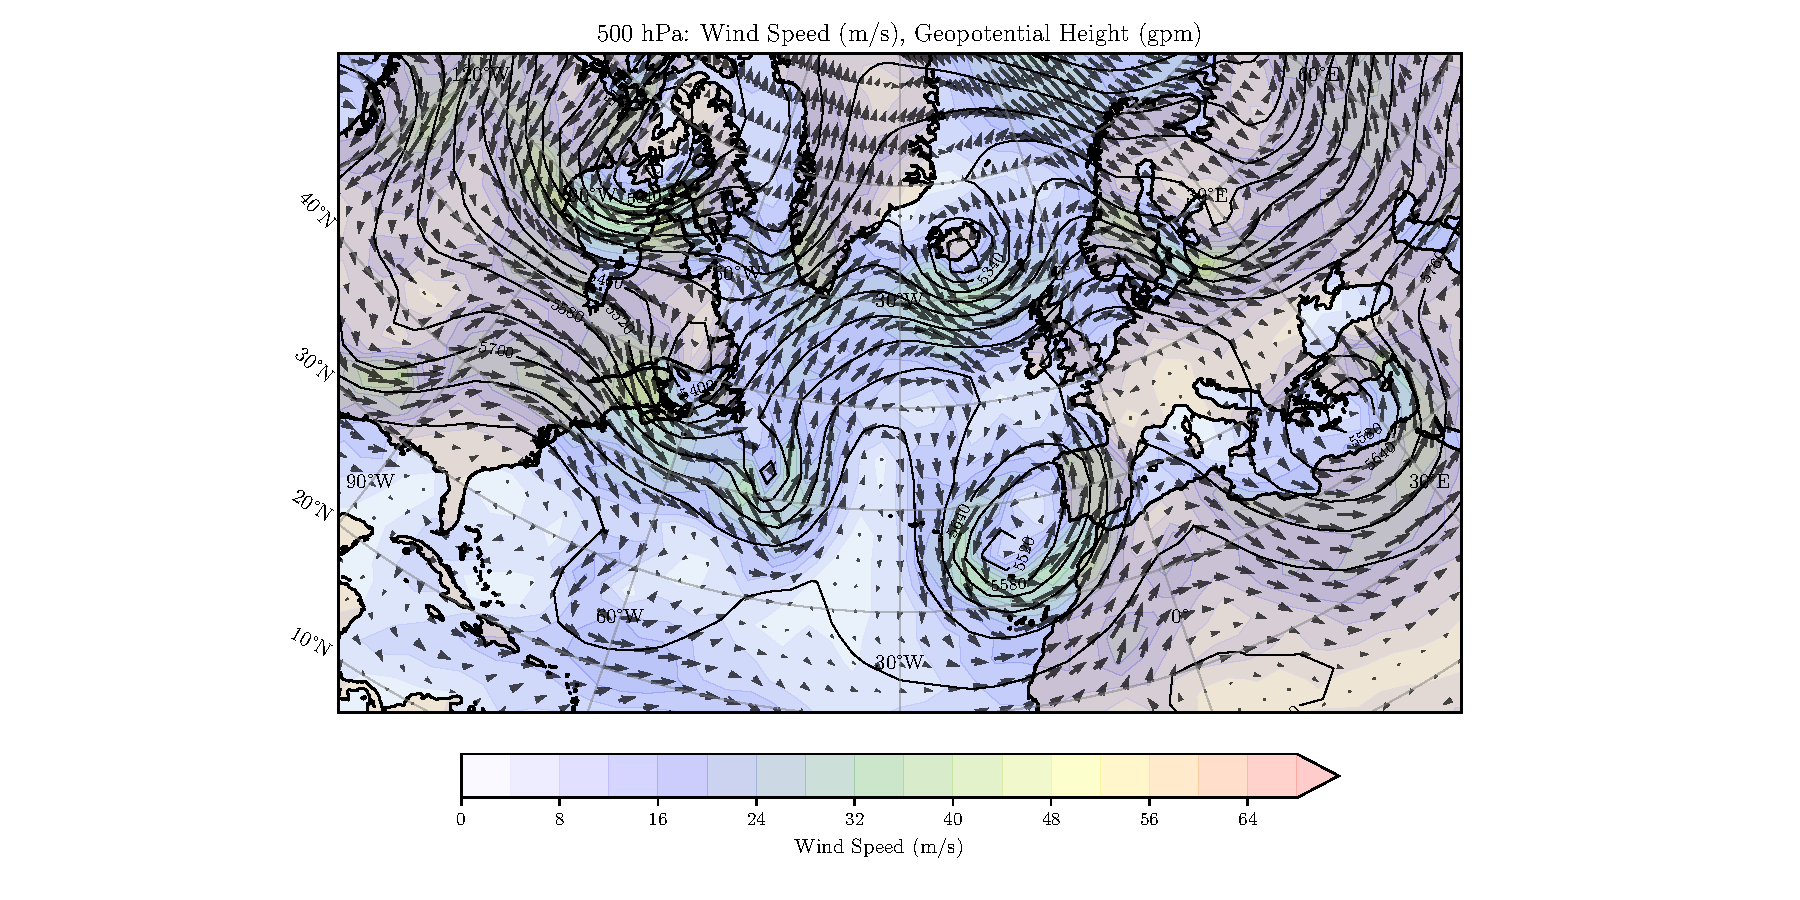
\includegraphics[width=\textwidth, trim=4cm 0cm 5cm 0cm, clip]{papers/rossby/images/weather/data_2025_5_1_00-00_500.pdf}
	\caption{Beispielkarte der Rossby-Wellenstruktur in 500\,hPa Höhe am 1.\ Mai 2025, 00:00~UTC.
		Projektion, Ausschnitt und inhaltliche Elemente wie im Text beschrieben.}
	\label{fig:rossby_atlantic_single}
\end{figure}

Nachdem das Beispielbild in Abbildung~\ref{fig:rossby_atlantic_single} die 
Darstellungselemente erläutert, betrachten wir nun eine Abfolge vom 1.\ bis 15.\ Mai~2025 
(Abbildung~\ref{fig:rossby_grid}), um die zeitliche Entwicklung der Rossby-Wellen 
nachzuvollziehen. Die Karten sind in 12-Stunden-Schritten angeordnet, sodass die 
wellenförmige Verlagerung und Verstärkung der Systeme deutlich erkennbar wird.


\begin{figure}
	\centering
	\renewcommand{\arraystretch}{0.5}
	\begin{tabular}{ccc}
		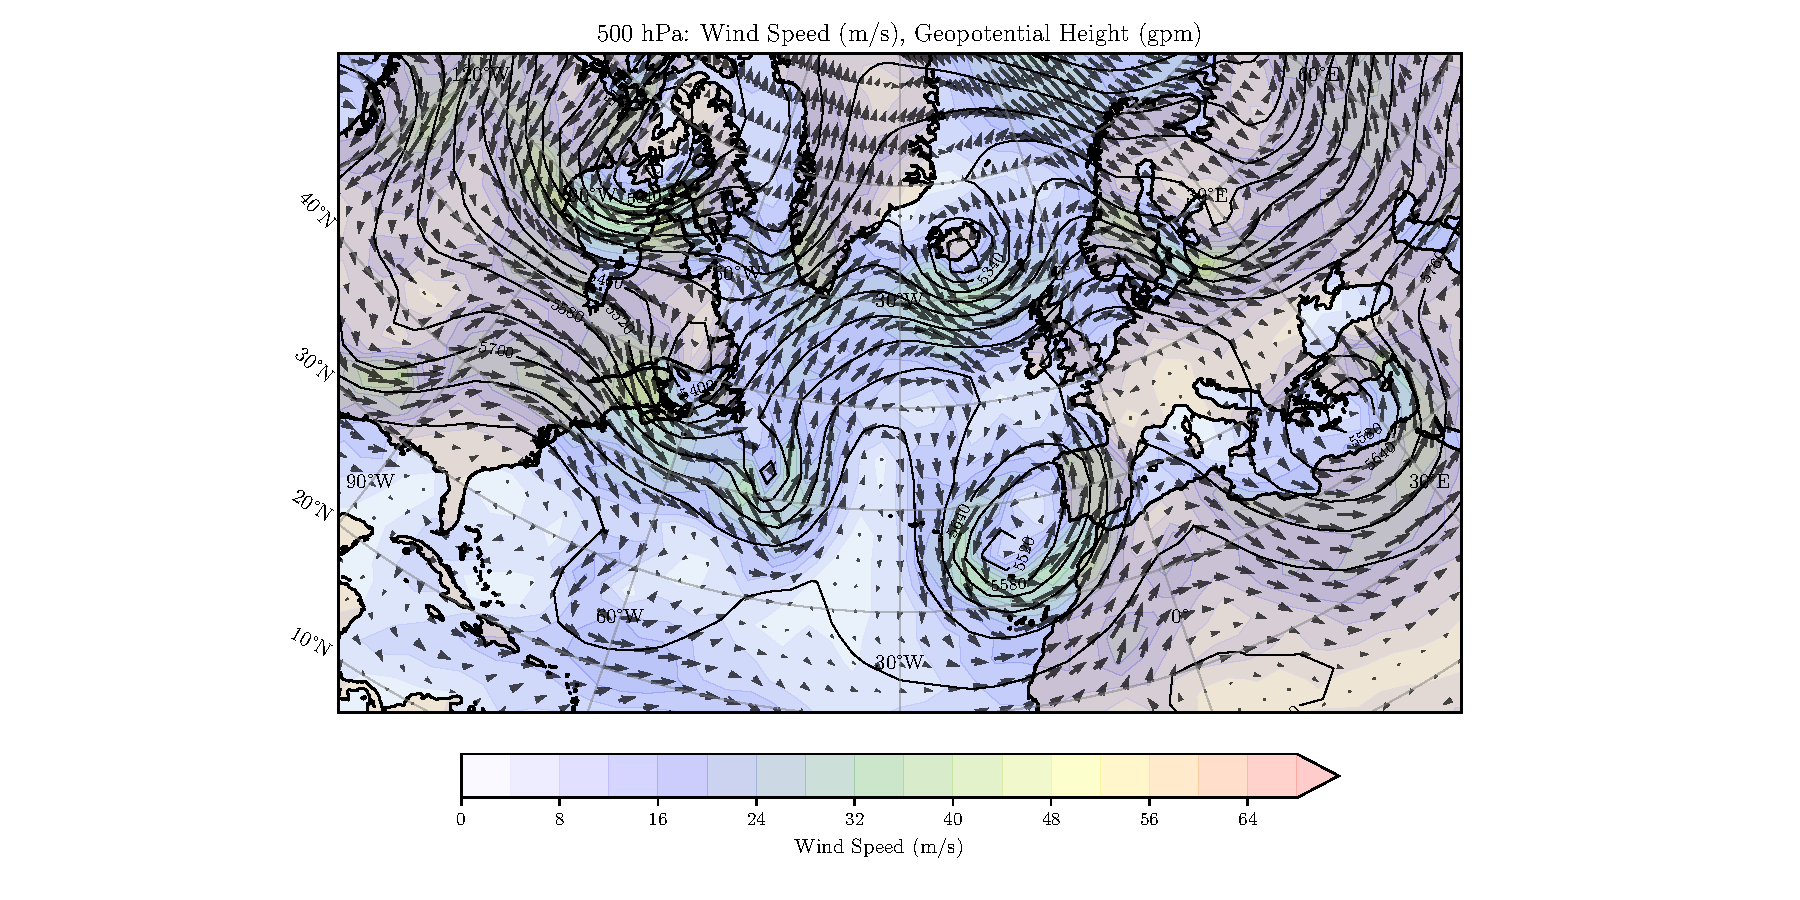
\includegraphics[width=0.32\textwidth, trim=5.75cm 3cm 5cm 0.9cm, clip]{papers/rossby/images/weather/data_2025_5_1_00-00_500.pdf} &
		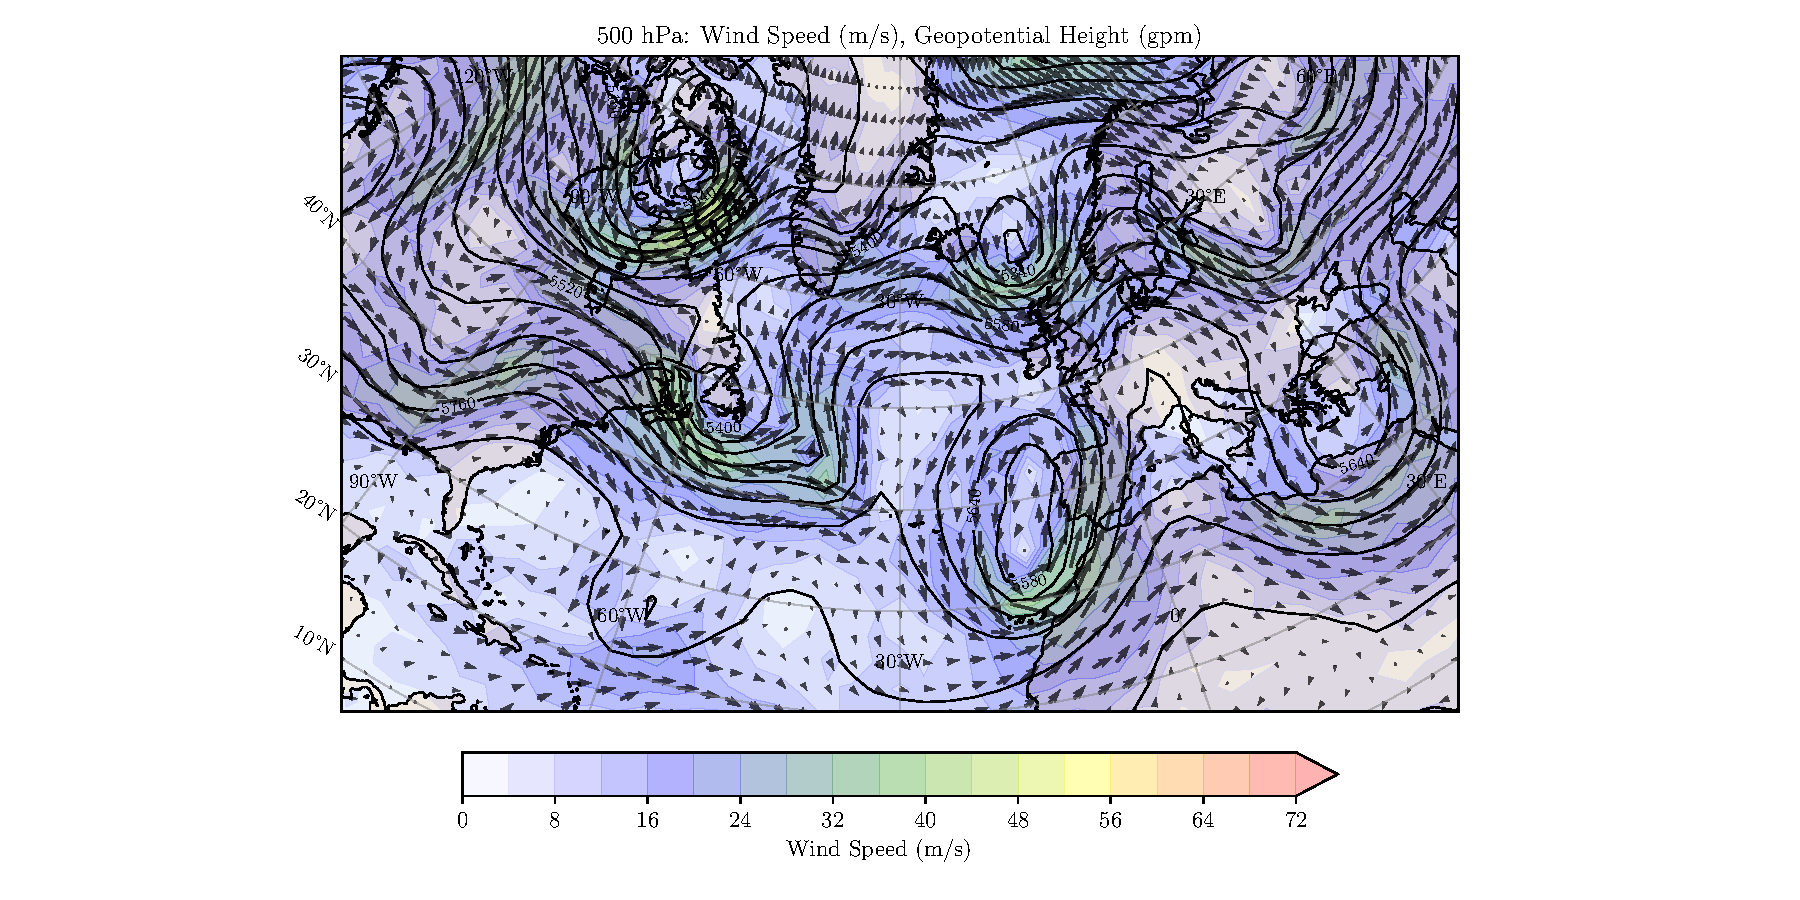
\includegraphics[width=0.32\textwidth, trim=5.75cm 3cm 5cm 0.9cm, clip]{papers/rossby/images/weather/data_2025_5_1_12-00_500.pdf} &
		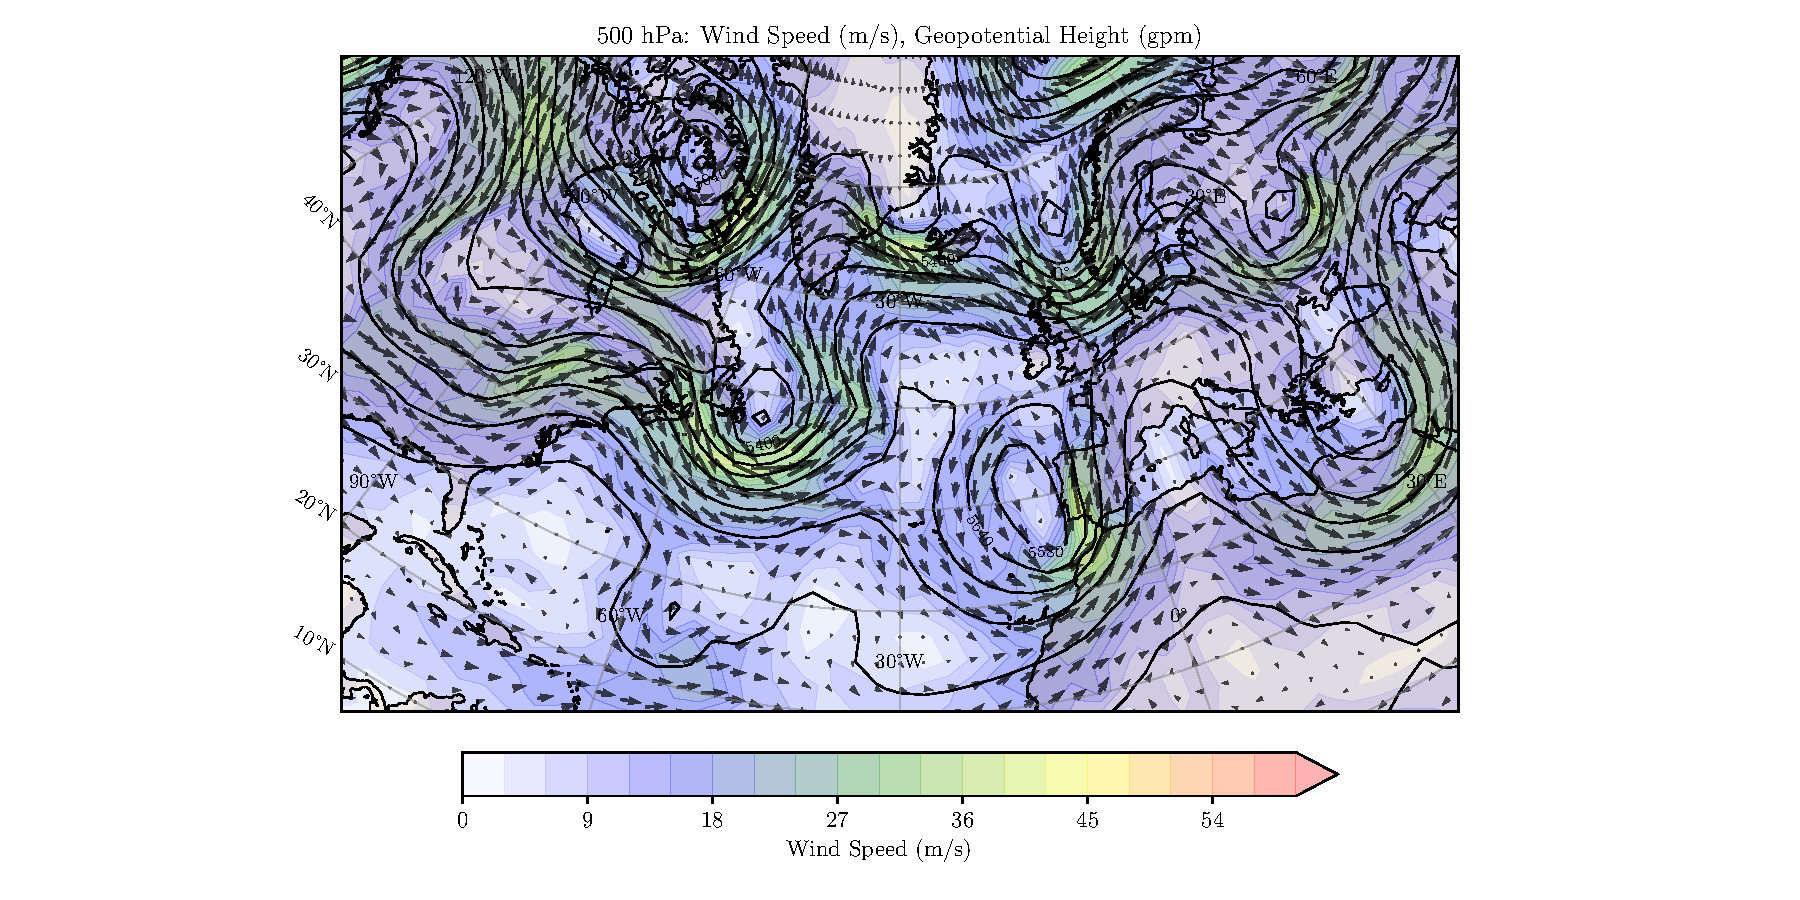
\includegraphics[width=0.32\textwidth, trim=5.75cm 3cm 5cm 0.9cm, clip]{papers/rossby/images/weather/data_2025_5_2_00-00_500.pdf}   \\
		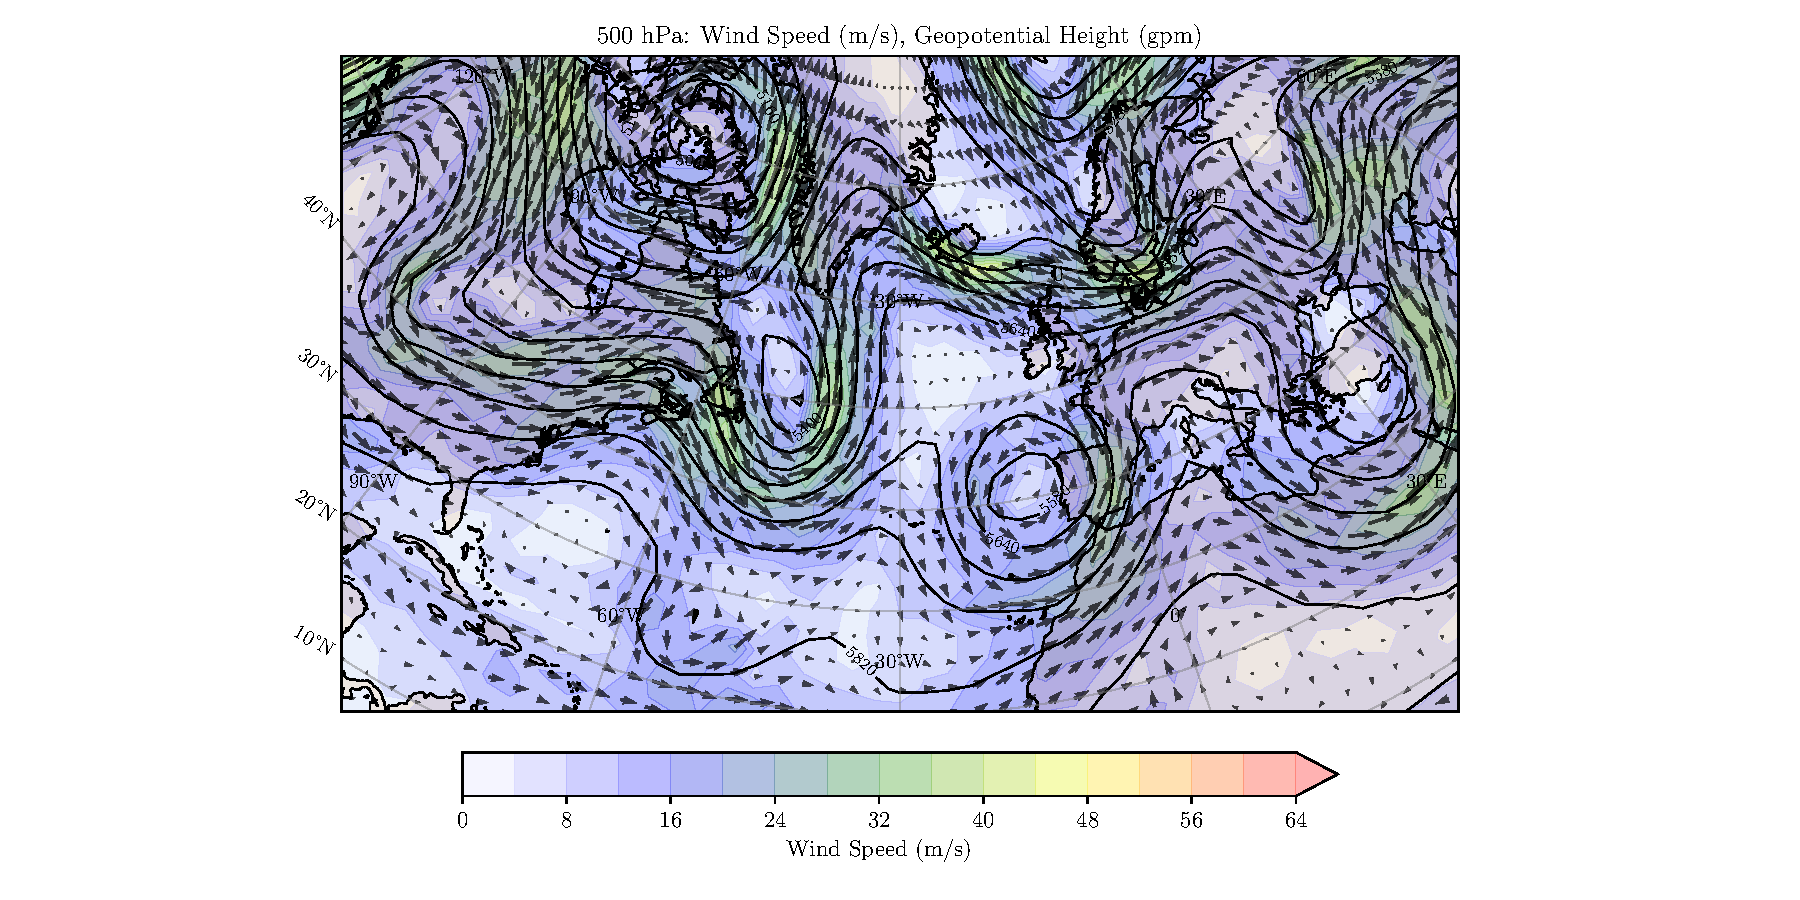
\includegraphics[width=0.32\textwidth, trim=5.75cm 3cm 5cm 0.9cm, clip]{papers/rossby/images/weather/data_2025_5_2_12-00_500.pdf} &
		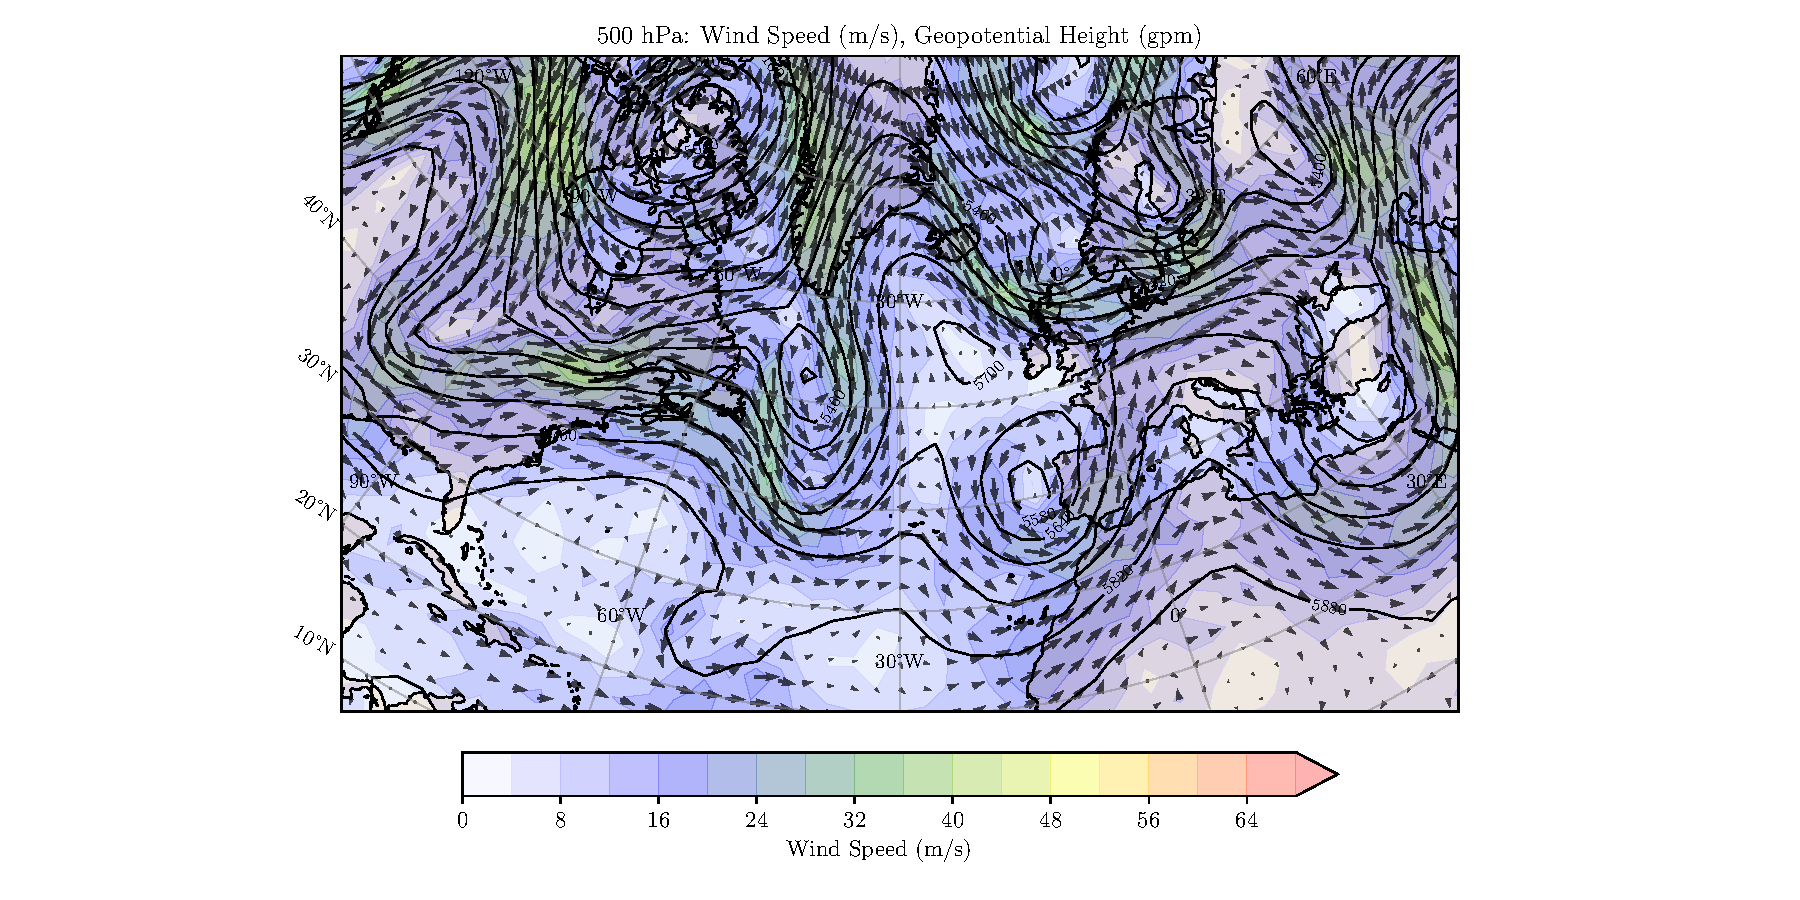
\includegraphics[width=0.32\textwidth, trim=5.75cm 3cm 5cm 0.9cm, clip]{papers/rossby/images/weather/data_2025_5_3_00-00_500.pdf} &
		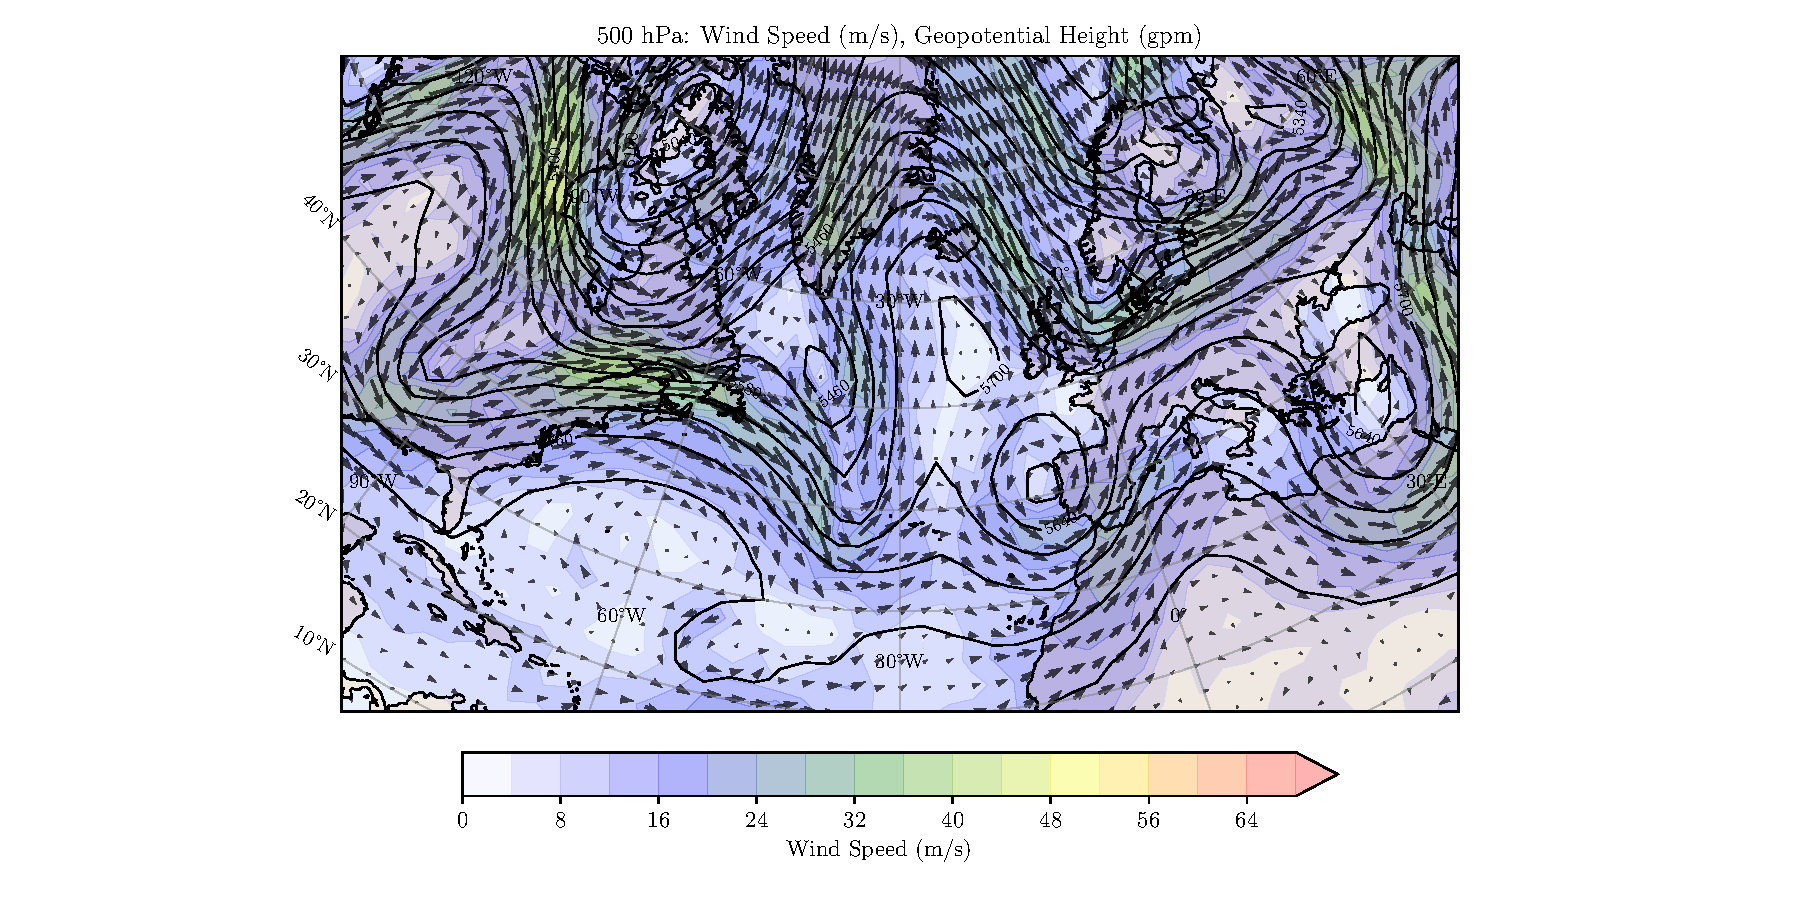
\includegraphics[width=0.32\textwidth, trim=5.75cm 3cm 5cm 0.9cm, clip]{papers/rossby/images/weather/data_2025_5_3_12-00_500.pdf}   \\
		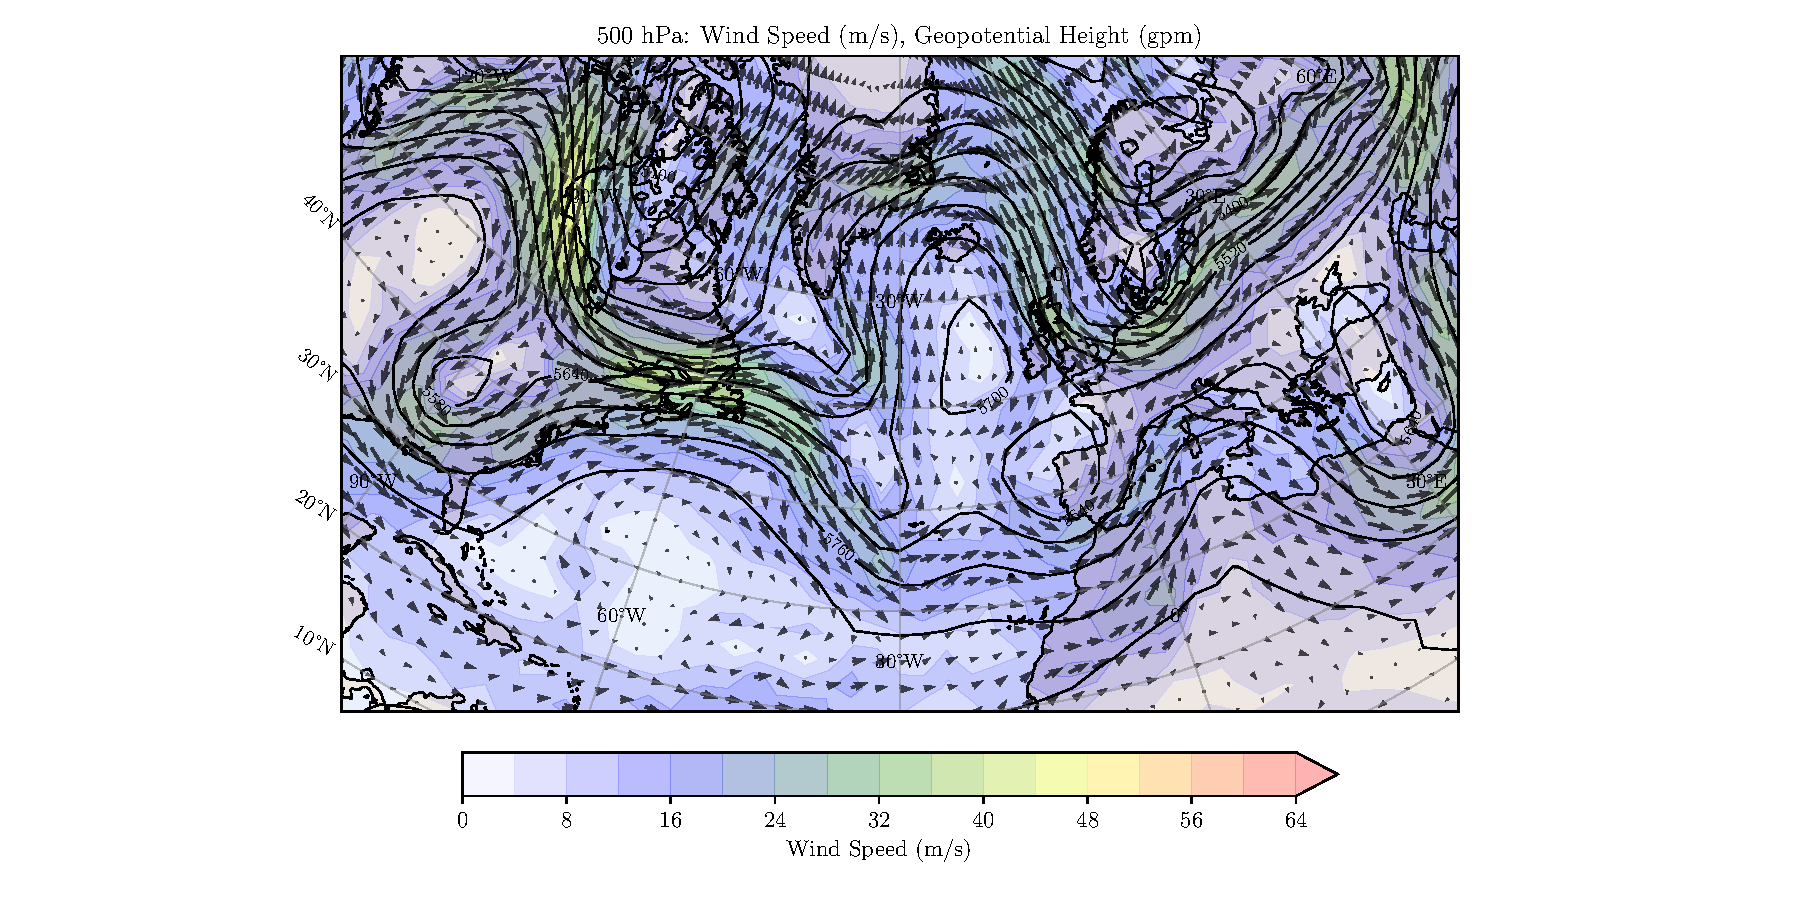
\includegraphics[width=0.32\textwidth, trim=5.75cm 3cm 5cm 0.9cm, clip]{papers/rossby/images/weather/data_2025_5_4_00-00_500.pdf} &
		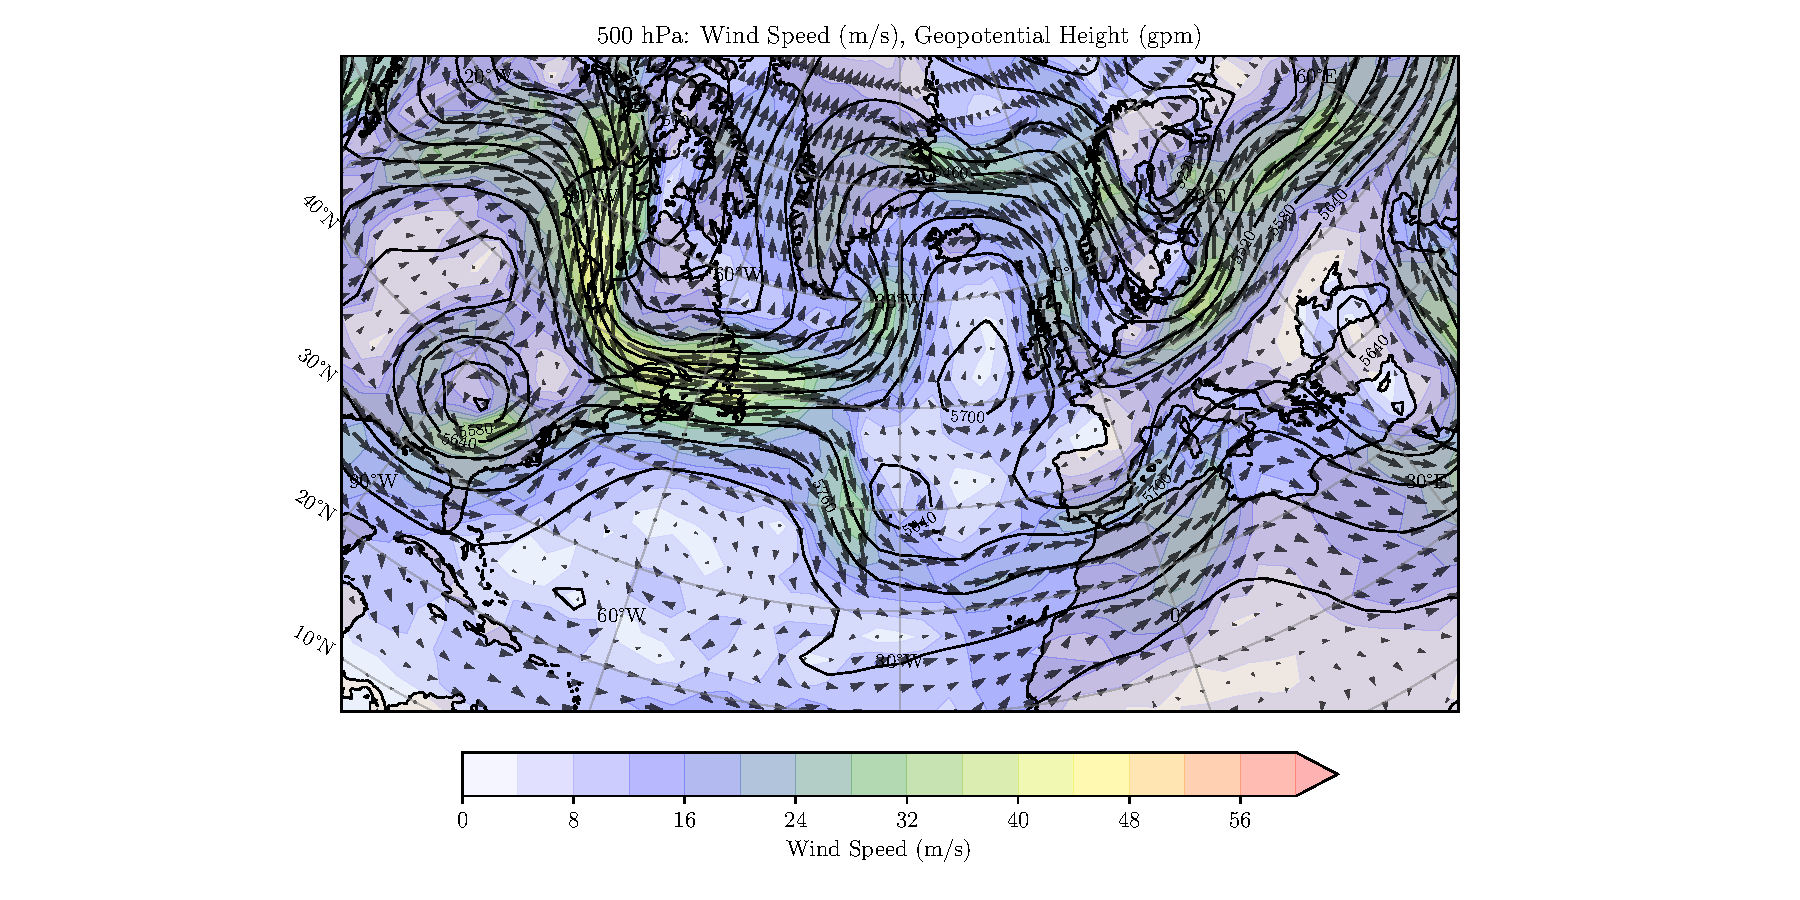
\includegraphics[width=0.32\textwidth, trim=5.75cm 3cm 5cm 0.9cm, clip]{papers/rossby/images/weather/data_2025_5_4_12-00_500.pdf} &
		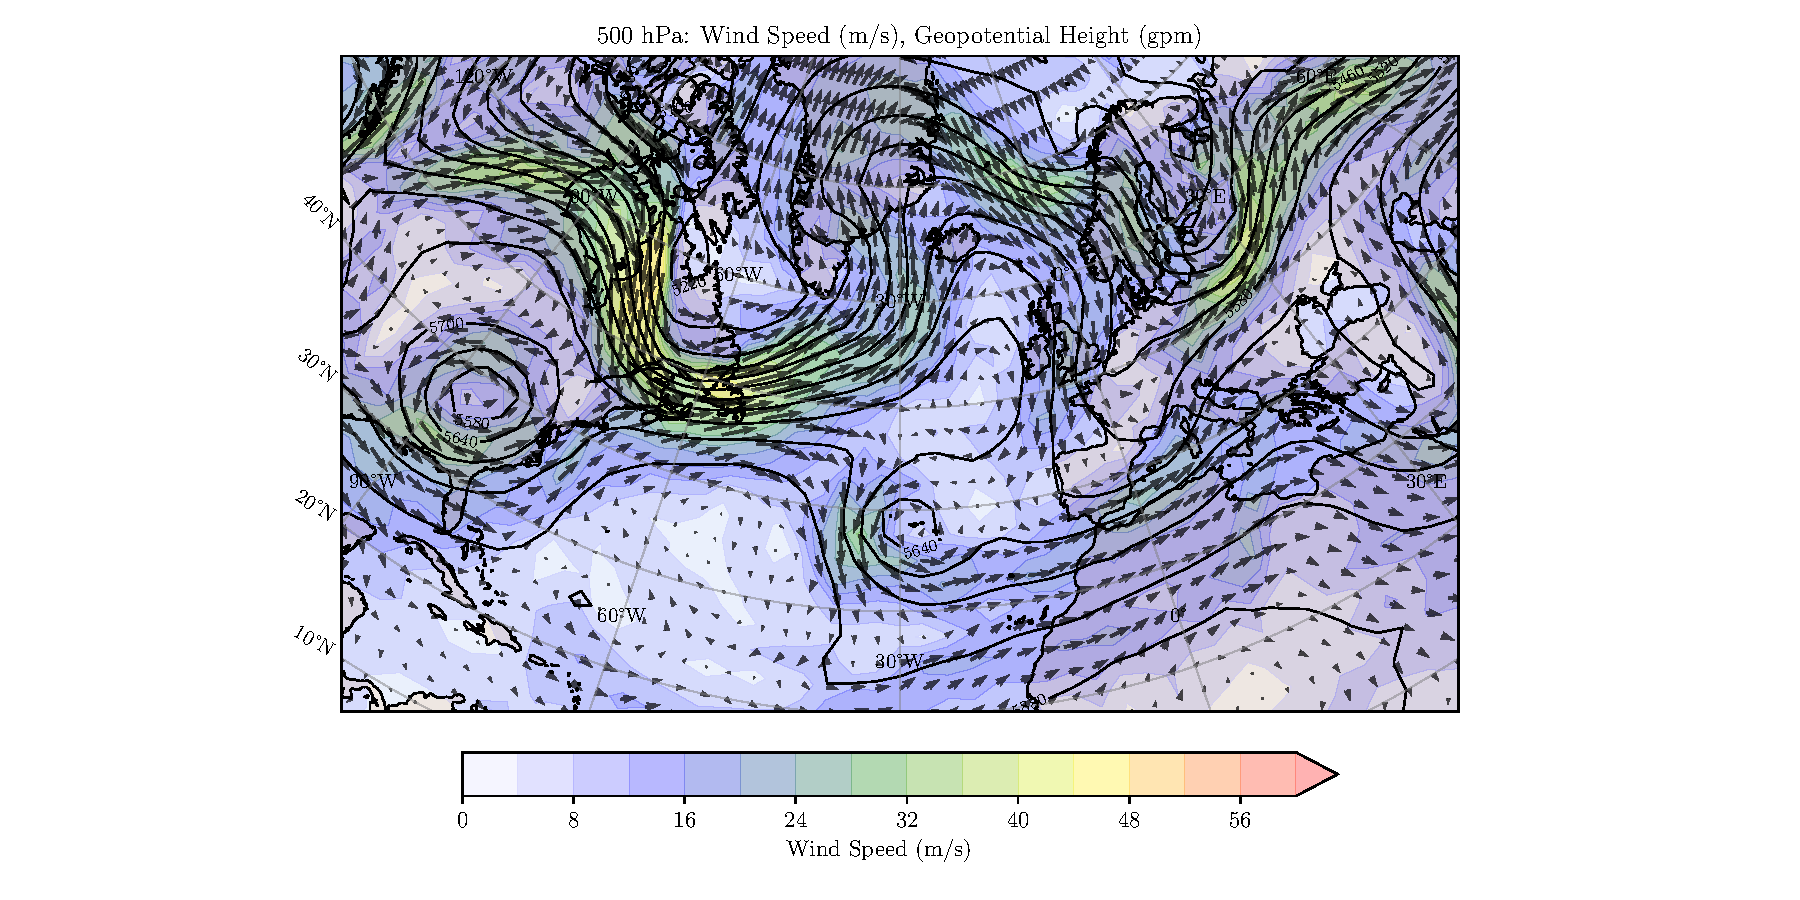
\includegraphics[width=0.32\textwidth, trim=5.75cm 3cm 5cm 0.9cm, clip]{papers/rossby/images/weather/data_2025_5_5_00-00_500.pdf}   \\
	\end{tabular}
	\caption{Abfolge der Rossby-Wellenstruktur in 500\,hPa Höhe vom 1.\ bis 15.\ Mai 2025 in 12-Stunden-Schritten.}
	\label{fig:rossby_grid}
\end{figure}

